\mychapter{Open Source Anonymous Credentials Library}

For Anonymous Credential and Privacy-Preserving Identity there is no library to help people learn the differences between constructions, what they can use or can't use and how they differ from a practical / functional implementation standpoint. 

Our contributions
1. built opensource library framework for SOTA anonymous credentials and benchmarked against each other in rust
2. Demonstrate that schnorr proofs which are usually "slandered" in academic papers for being linear in the size of the proven attributed are in-fact sublinear in practice due to MSM techniques
3. we show the speedup from batch / windowing schnorr proofs 
4. Show the computation reduction in pairings when using miller loop intermediate computation rather than computing and epxonentiating GT points



\section{Practical Proof Analysis}
\subsection{Sigma Protocols}\label{sigma-protocol-analysis}
Many schemes refer to sigma protocol as having linear size proofs. 
While this is true in theory, using multi-scalar-multiplication, a popular algorithm in many cryptographic libraries, we show that sigma protocols are, in fact, sublinear rather than linear when message size doubles.

These findings support the hypothesis that practical efficiency is substantially better than theoretical complexity would suggest when using MSM in Schnorr protocols and thus the proof protocols in PS and BBS+ based anonymous credentials are sublinear in practice.

\begin{figure}
    \centering
    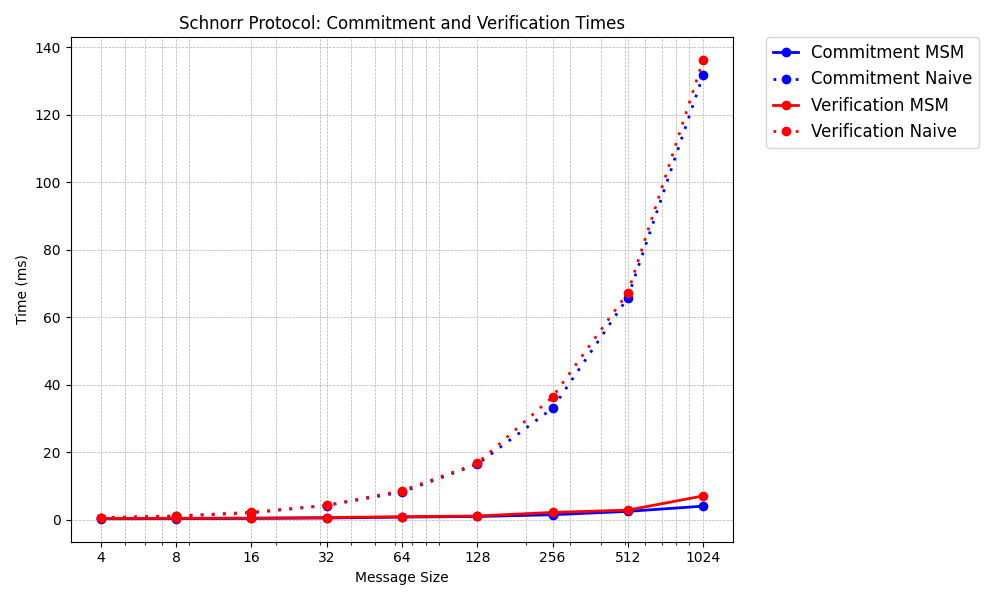
\includegraphics[width=0.75\linewidth]{schnorr_msm_no_msm.png}
    \caption{Schnorr Protocol - Practical Benchmarks with Multi-Scalar Multiplication}
    \label{fig:schnorr-benchmarks}
\end{figure}




\subsection{Pairing Protocols}

\begin{figure}
    \centering
    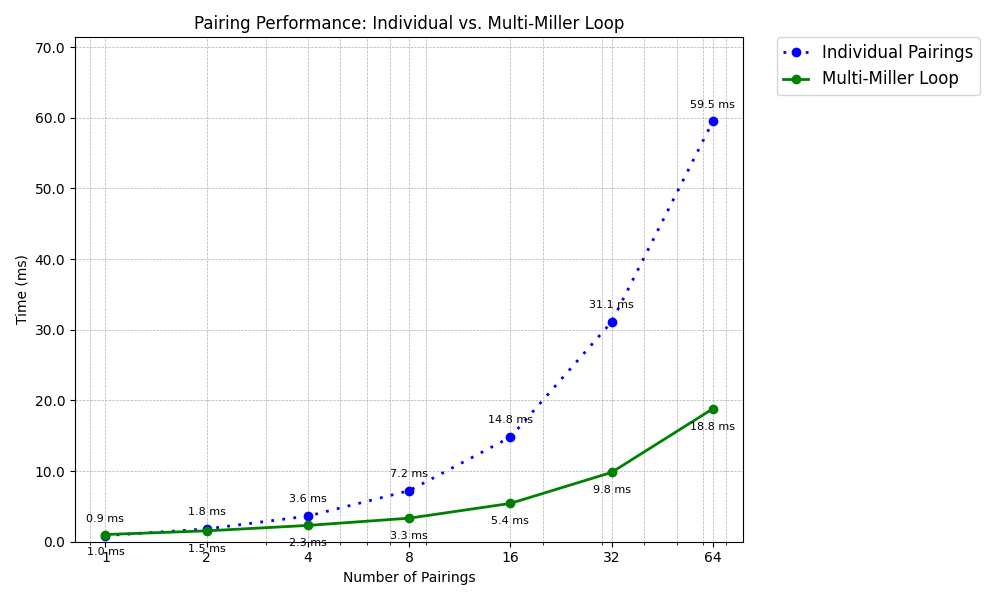
\includegraphics[width=0.75\linewidth]{pairing_comparison.png}
        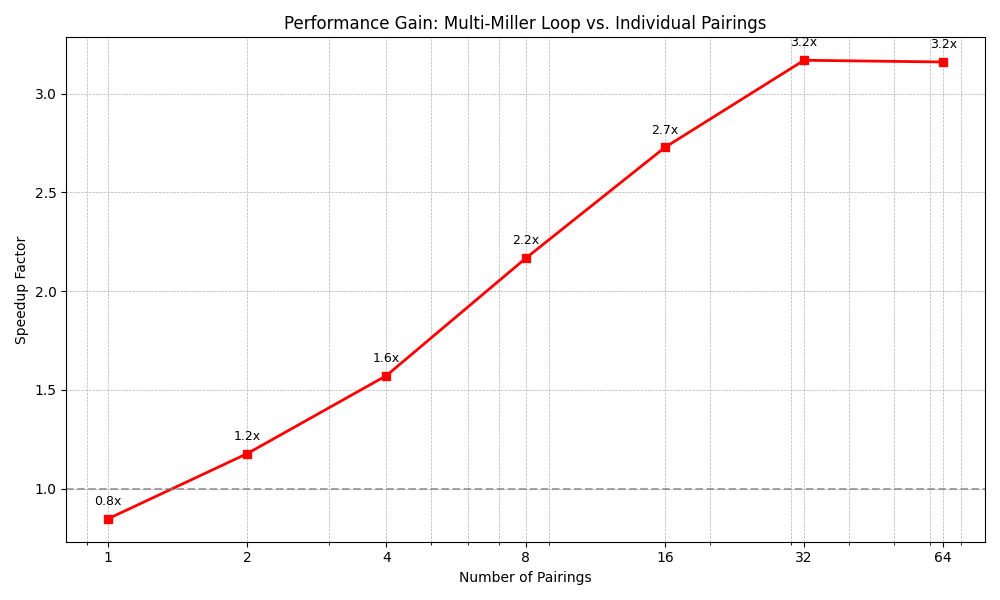
\includegraphics[width=0.75\linewidth]{pairing_comparison2.png}
    \caption{Elliptic Curve Pairings - Practical Benchmarks with Miller-Loop Intermediate Computation}
    \label{fig:enter-label}
\end{figure}
